
%%%%%%%%%%%%%%%%%%%%%%%%%%%%%%%%%%%%%%%%%%%%%%%%%%%%%%%%
%
% Copyright (c) 2003-2010 by University of Queensland
% Earth Systems Science Computational Center (ESSCC)
% http://www.uq.edu.au/esscc
%
% Primary Business: Queensland, Australia
% Licensed under the Open Software License version 3.0
% http://www.opensource.org/licenses/osl-3.0.php
%
%%%%%%%%%%%%%%%%%%%%%%%%%%%%%%%%%%%%%%%%%%%%%%%%%%%%%%%%

\begin{figure}[h!]
\centerline{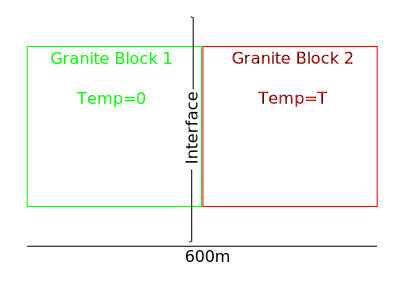
\includegraphics[width=4.in]{figures/onedheatdiff001}}
\caption{Temperature differential along a single interface between two granite blocks.}
\label{fig:onedgbmodel}
\end{figure}

\section{One Dimensional Heat Diffusion in Granite}
\label{Sec:1DHDv00}

The first model consists of two blocks of isotropic material, for instance granite, sitting next to each other.
Initially, \textit{Block 1} is of a temperature
\verb|T1| and \textit{Block 2} is at a temperature \verb|T2|.
We assume that the system is insulated.
What would happen to the temperature distribution in each block over time? 
Intuition tells us that heat will transported from the hotter block to the cooler until both
blocks have the same temperature.

\subsection{1D Heat Diffusion Equation}
We can model the heat distribution of this problem over time using the one dimensional heat diffusion equation\footnote{A detailed discussion on how the heat diffusion equation is derived can be found at \url{http://online.redwoods.edu/instruct/darnold/DEProj/sp02/AbeRichards/paper.pdf}};
which is defined as:
\begin{equation}
\rho c\hackscore p \frac{\partial T}{\partial t} - \kappa \frac{\partial^{2} T}{\partial x^{2}} = q\hackscore H 
\label{eqn:hd}
\end{equation}
where $\rho$ is the material density, $c\hackscore p$ is the specific heat and $\kappa$ is the thermal 
conductivity\footnote{A list of some common thermal conductivities is available from Wikipedia \url{http://en.wikipedia.org/wiki/List_of_thermal_conductivities}}. Here we assume that these material 
parameters are \textbf{constant}. 
The heat source is defined by the right hand side of \refEq{eqn:hd} as $q\hackscore{H}$; this can take the form of a constant or a function of time and space. For example $q\hackscore{H} = q\hackscore{0}e^{-\gamma t}$ where we have the output of our heat source decaying with time. There are also two partial derivatives in \refEq{eqn:hd}; $\frac{\partial T}{\partial t}$ describes the change in temperature with time while $\frac{\partial ^2 T}{\partial x^2}$ is the spatial change of temperature. As there is only a single spatial dimension to our problem, our temperature solution $T$ is only dependent on the time $t$ and our position along the iron bar $x$.

\subsection{PDEs and the General Form}
Potentially, it is now possible to solve PDE \refEq{eqn:hd} analytically and this would produce an exact solution to our problem. However, it is not always possible or practical to solve a problem this way. Alternatively, computers can be used to solve these kinds of problems. To do this, a numerical approach is required to discretised 
the PDE \refEq{eqn:hd} in time and space so finally we are left with a finite number of equations for a finite number of spatial and time steps in the model. While discretization introduces approximations and a degree of error, we find that a sufficiently sampled model is generally accurate enough for the requirements of the modeller.

Firstly, we will discretise the PDE \refEq{eqn:hd} in the time direction which will
leave as with a steady linear PDE which is involving spatial derivatives only and needs to be solved in each time 
step to progress in time - \esc can help us here.

For the discretization in time we will use is the Backwards Euler approximation scheme\footnote{see \url{http://en.wikipedia.org/wiki/Euler_method}}. It bases on the
approximation 
\begin{equation}
\frac{\partial T(t)}{\partial t} \approx \frac{T(t)-T(t-h)}{h}
\label{eqn:beuler}
\end{equation}
for  $\frac{\partial T}{\partial t}$  at time $t$ 
where $h$ is the time step size. This can also be written as;
\begin{equation}
\frac{\partial T}{\partial t}(t^{(n)}) \approx \frac{T^{(n)} - T^{(n-1)}}{h}
\label{eqn:Tbeuler}
\end{equation}
where the upper index $n$ denotes the n\textsuperscript{th} time step. So one has
\begin{equation}
\begin{array}{rcl}
t^{(n)} & = & t^{(n-1)}+h \\
T^{(n)} & = & T(t^{(n-1)}) \\ 
\end{array}
\label{eqn:Neuler}
\end{equation}
Substituting \refEq{eqn:Tbeuler} into \refEq{eqn:hd} we get;
\begin{equation}
\frac{\rho c\hackscore p}{h} (T^{(n)} - T^{(n-1)}) - \kappa \frac{\partial^{2} T^{(n)}}{\partial x^{2}} = q\hackscore H 
\label{eqn:hddisc}
\end{equation}
Notice that we evaluate the spatial derivative term at current time $t^{(n)}$ - therefore the name \textbf{backward Euler} scheme. Alternatively, one can use evaluate the spatial derivative term at the previous time $t^{(n-1)}$. This 
approach is called the \textbf{forward Euler} scheme. This scheme can provide some computational advantages which
we are not discussed here but has the major disadvantage that depending on the 
material parameter as well as the discretization of the spatial derivative term the time step size $h$ needs to be chosen sufficiently small to achieve a stable temperature when progressing in time. The term \textit{stable} means
that the approximation of the temperature will not grow beyond its initial bounds and becomes non-physical. 
The backward Euler which we use here is unconditionally stable meaning that under the assumption of
physically correct problem set-up the temperature approximation remains physical for all times. 
The user needs to keep in mind that the discretization error introduced by \refEq{eqn:beuler} 
is sufficiently small so a good approximation of the true temperature is calculated. It is
therefore crucial that the user remains critical about his/her results and for instance compares 
the results for different time and spatial step sizes. 

To get the temperature $T^{(n)}$ at time $t^{(n)}$ we need to solve the linear 
differential equation \refEq{eqn:hddisc} which is only including spatial derivatives. To solve this problem
we want to to use \esc. 

\esc interfaces with any given PDE via a general form. For the purpose of this introduction we will illustrate a simpler version of the full linear PDE general form which is available in the \esc user's guide. A simplified form that suits our heat diffusion problem\footnote{In the form of the \esc users guide which using the Einstein convention is written as 
$-(A\hackscore{jl} u\hackscore{,l})\hackscore{,j}+D u =Y$}
is described by;
\begin{equation}\label{eqn:commonform nabla}
-\nabla\cdot(A\cdot\nabla u) + Du = f
\end{equation}
where $A$, $D$ and $f$ are known values and $u$ is the unknown solution. The symbol $\nabla$ which is called the \textit{Nabla operator} or \textit{del operator} represents
the spatial derivative of its subject - in this case $u$. Lets assume for a moment that we deal with a one-dimensional problem then ;
\begin{equation}
\nabla = \frac{\partial}{\partial x}
\end{equation}
and we can write \refEq{eqn:commonform nabla} as;
\begin{equation}\label{eqn:commonform}
-A\frac{\partial^{2}u}{\partial x^{2}} + Du = f
\end{equation}
if $A$ is constant. To match this simplified general form to our problem \refEq{eqn:hddisc} 
we rearrange \refEq{eqn:hddisc};
\begin{equation}
\frac{\rho c\hackscore p}{h} T^{(n)} - \kappa \frac{\partial^2 T^{(n)}}{\partial x^2} = q\hackscore H +  \frac{\rho c\hackscore p}{h} T^{(n-1)}
\label{eqn:hdgenf}
\end{equation}
The PDE is now in a form that satisfies \refEq{eqn:commonform nabla} which is required for \esc to solve our PDE. This can be done by generating a solution for successive increments in the time nodes $t^{(n)}$ where 
$t^{(0)}=0$ and  $t^{(n)}=t^{(n-1)}+h$ where $h>0$ is the step size and assumed to be constant. 
In the following the upper index ${(n)}$ refers to a value at time $t^{(n)}$. Finally, by comparing \refEq{eqn:hdgenf} with \refEq{eqn:commonform} it can be seen that;
\begin{equation}\label{ESCRIPT SET}
u=T^{(n)}; 
A = \kappa; D = \frac{\rho c \hackscore{p}}{h}; f = q \hackscore{H} + \frac{\rho c\hackscore p}{h} T^{(n-1)}
\end{equation}

\subsection{Boundary Conditions}
\label{SEC BOUNDARY COND}
With the PDE sufficiently modified, consideration must now be given to the boundary conditions of our model. Typically there are two main types of boundary conditions known as \textbf{Neumann} and \textbf{Dirichlet} boundary conditions\footnote{More information on Boundary Conditions is available at Wikipedia \url{http://en.wikipedia.org/wiki/Boundary_conditions}}, respectively. 
A \textbf{Dirichlet boundary condition} is conceptually simpler and is used to prescribe a known value to the unknown - in our example the temperature - on parts of the boundary or on the entire boundary of the region of interest. 
We discuss Dirichlet boundary condition in our second example presented in Section~\ref{Sec:1DHDv0}.

We make the model assumption that the system is insulated so we need
to add an appropriate boundary condition to prevent
any loss or inflow of energy at boundary of our domain. Mathematically this is expressed by prescribing
the heat flux $\kappa \frac{\partial T}{\partial x}$  to zero. In our simplified one dimensional model this is expressed
in the form;
\begin{equation}
\kappa \frac{\partial T}{\partial x}  = 0 
\end{equation}
or in a more general case as
\begin{equation}\label{NEUMAN 1}
\kappa \nabla T \cdot n  = 0 
\end{equation}
where $n$  is the outer normal field \index{outer normal field} at the surface of the domain. 
The $\cdot$ (dot) refers to the  dot product of the vectors $\nabla T$ and $n$. In fact, the term $\nabla T \cdot n$ is the normal derivative of 
the temperature $T$. Other notations which are used are\footnote{The \esc notation for the normal
derivative is $T\hackscore{,i} n\hackscore i$.};
\begin{equation}
\nabla T \cdot n  = \frac{\partial T}{\partial n} \; .
\end{equation}
A condition of the type \refEq{NEUMAN 1} defines a \textbf{Neuman boundary condition} for the PDE. 

The PDE \refEq{eqn:hdgenf} 
and the Neuman boundary condition~\ref{eqn:hdgenf} (potentially together with the Dirichlet boundary condition set)  define a \textbf{boundary value problem}. 
It is a nature of a boundary value problem that it allows to make statements on the solution in the
interior of the domain from information known on the boundary only. In most cases
we use the term partial differential equation but in fact mean a boundary value problem. 
It is important to keep in mind that boundary conditions need to be complete and consistent in the sense that 
at any point on the boundary either a Dirichlet or a Neuman boundary condition must be set.

Conveniently, \esc makes default assumption on the boundary conditions which the user may modify where appropriate. 
For a problem of the form in~\refEq{eqn:commonform nabla} the default condition\footnote{In the form of the \esc users guide which is using the Einstein convention is written as 
$n\hackscore{j}A\hackscore{jl} u\hackscore{,l}=0$.} is;
\begin{equation}\label{NEUMAN 2}
n\cdot A \cdot\nabla u = 0 
\end{equation}
which is used everywhere on the boundary. Again $n$ denotes the outer normal field. 
Notice that the coefficient $A$ is the same as in the \esc PDE~\ref{eqn:commonform nabla}. 
With the settings for the coefficients we have already identified in \refEq{ESCRIPT SET} this
condition translates into 
\begin{equation}\label{NEUMAN 2b}
\kappa \frac{\partial T}{\partial x} = 0 
\end{equation}
for the boundary of the domain. This is identical to the Neuman boundary condition we want to set. \esc will take care of this condition for us. We will discuss the Dirichlet boundary condition later.

\subsection{Outline of the Implementation}
\label{sec:outline}
To solve the heat diffusion equation (equation \refEq{eqn:hd}) we will write a simple \pyt script. At this point we assume that you have some basic understanding of the \pyt programming language. If not there are some pointers and links available in Section \ref{sec:escpybas}. The script we will discuss later in details will have four major steps. Firstly we need to define the domain where we want to 
calculate the temperature. For our problem this is the joint blocks of granite which has a rectangular shape. Secondly we need to define the PDE 
we need to solve in each time step to get the updated temperature. Thirdly we need to define the the coefficients of the PDE and finally we need to solve the PDE. The last two steps need to be repeated until the final time marker has been reached. As a work flow this takes the form;
\begin{enumerate}
 \item create domain
 \item create PDE
 \item while end time not reached:
\begin{enumerate}
 \item set PDE coefficients
 \item solve PDE
 \item update time marker
\end{enumerate}
\item end of calculation
\end{enumerate}
In the terminology of \pyt the domain and PDE are represented by \textbf{objects}. The nice feature of an object is that it defined by it usage and features
rather than its actual representation. So we will create a domain object to describe the geometry of the two
granite blocks. The main feature 
of the object we will use is the fact that we can define PDEs and spatially distributed values such as the temperature 
on a domain. In fact the domain object has many more features - most of them you will 
never use and do not need to understand. Similar a PDE object is defined by the fact that we can define the coefficients of the PDE and solve the PDE. At a 
later stage you may use more advanced features of the PDE class but you need to worry about them only at the point when you use them.


\begin{figure}[t]
 \centering
   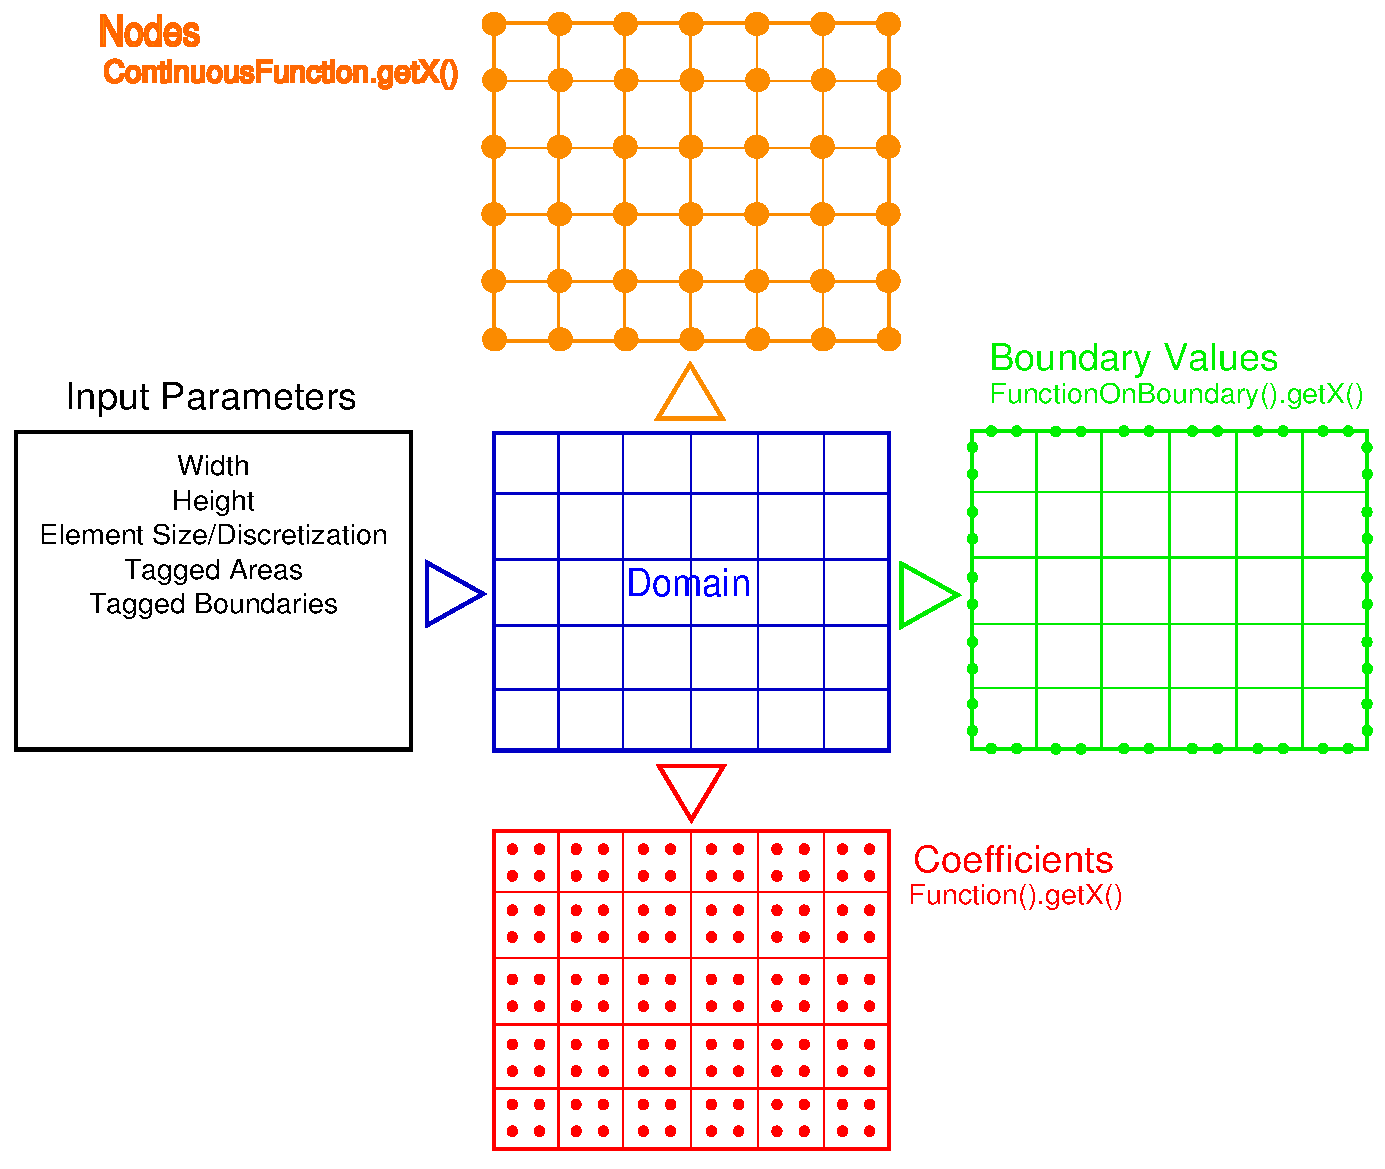
\includegraphics[width=6in]{figures/functionspace.pdf}
   \label{fig:fs}
   \caption{\esc domain construction overview}
\end{figure}

\subsection{The Domain Constructor in \esc}
\label{ss:domcon}
It is helpful to have a better understanding how spatially distributed value such as the temperature or PDE coefficients are interpreted in \esc. Again
from the user's point of view the representation of these spatially distributed values is not relevant. 

There are various ways to construct domain objects. The simplest form is as rectangular shaped region with a length and height. There is
a ready to use function call for this. Besides the spatial dimensions the function call will require you to specify the number
elements or cells to be used along the length and height, see \reffig{fig:fs}. Any spatially distributed value 
and the PDE is represented in discrete form using this element representation\footnote{We will use the finite element method (FEM), see \url{http://en.wikipedia.org/wiki/Finite_element_method} for details.}. Therefore we will have access to an approximation of the true PDE solution only. 
The quality of the approximation depends - besides other factors- mainly on the number of elements being used. In fact, the 
approximation becomes better the more elements are used. However, computational costs and compute time grow with the number of
elements being used. It therefore important that you find the right balance between the demand in accuracy and acceptable resource usage.

In general, one can thinks about a domain object as a composition of nodes and elements. 
As shown in \reffig{fig:fs}, an element is defined by the nodes used to describe its vertices. 
To represent spatial distributed values the user can use 
the values at the nodes, at the elements in the interior of the domain or at elements located at the surface of the domain. 
The different approach used to represent values is called \textbf{function space} and is attached to all objects
in \esc representing a spatial distributed value such as the solution of a PDE. The three 
function spaces we will use at the moment are;
\begin{enumerate}
\item the nodes, called by \verb|ContinuousFunction(domain)| ;
\item the elements/cells, called by \verb|Function(domain)| ; and
\item the boundary, called by \verb|FunctionOnBoundary(domain)| .
\end{enumerate}
A function space object such as \verb|ContinuousFunction(domain)| has the method \verb|getX| attached to it. This method returns the
location of the so-called \textbf{sample points} used to represent values with the particular function space attached to it. So the
call \verb|ContinuousFunction(domain).getX()| will return the coordinates of the nodes used to describe the domain while
the  \verb|Function(domain).getX()| returns the coordinates of numerical integration points within elements, see
\reffig{fig:fs}. 

This distinction between different representations of spatial distributed values 
is important in order to be able to vary the degrees of smoothness in a PDE problem. 
The coefficients of a PDE need not be continuous thus this qualifies as a \verb|Function()| type. 
On the other hand a temperature distribution must be continuous and needs to be represented with a \verb|ContinuousFunction()| function space.
An influx may only be defined at the boundary and is therefore a \verb FunctionOnBoundary()  object.  
\esc allows certain transformations of the function spaces. A \verb ContinuousFunction()  can be transformed into a \verb|FunctionOnBoundary()|
or \verb|Function()|. On the other hand there is not enough information in a \verb FunctionOnBoundary()  to transform it to a \verb ContinuousFunction()  .
These transformations, which are called \textbf{interpolation} are invoked automatically by \esc if needed.

Later in this introduction we will discuss how
to define specific areas of geometry with different materials which are represented by different material coefficients such the
thermal conductivities $kappa$. A very powerful technique to define these types of PDE 
coefficients is tagging. Blocks of materials and boundaries can be named and values can be defined on subregions based on their names.
This is simplifying PDE coefficient and flux definitions. It makes for much easier scripting. We will discuss this technique in Section~\ref{STEADY-STATE HEAT REFRACTION}.


\subsection{A Clarification for the 1D Case}
It is necessary for clarification that we revisit the general PDE from \refeq{eqn:commonform nabla} under the light of a two dimensional domain. \esc is inherently designed to solve problems that are greater than one dimension and so \refEq{eqn:commonform nabla} needs to be read as a higher dimensional problem. In the case of two spatial dimensions the \textit{Nabla operator} has in fact two components $\nabla = (\frac{\partial}{\partial x}, \frac{\partial}{\partial y})$. In full, \refEq{eqn:commonform nabla} assuming a constant coefficient $A$, takes the form;
\begin{equation}\label{eqn:commonform2D}
-A\hackscore{00}\frac{\partial^{2}u}{\partial x^{2}} 
-A\hackscore{01}\frac{\partial^{2}u}{\partial x\partial y} 
-A\hackscore{10}\frac{\partial^{2}u}{\partial y\partial x} 
-A\hackscore{11}\frac{\partial^{2}u}{\partial y^{2}} 
+ Du = f
\end{equation}
Notice that for the higher dimensional case $A$ becomes a matrix. It is also
important to notice that the usage of the Nabla operator creates
a compact formulation which is also independent from the spatial dimension. 
So to make the general PDE \refEq{eqn:commonform2D} one dimensional as
shown in \refEq{eqn:commonform} we need to set
\begin{equation}
A\hackscore{00}=A; A\hackscore{01}=A\hackscore{10}=A\hackscore{11}=0
\end{equation}


\subsection{Developing a PDE Solution Script}
\label{sec:key}
\sslist{onedheatdiffbase.py}
We will write a simple \pyt script which uses the \modescript, \modfinley and \modmpl modules. 
By developing a script for \esc, the heat diffusion equation can be solved at successive time steps for a predefined period using our general form \refEq{eqn:hdgenf}. Firstly it is necessary to import all the libraries\footnote{The libraries contain predefined scripts that are required to solve certain problems, these can be simple like sine and cosine functions or more complicated like those from our \esc library.} 
that we will require.
\begin{python}
from esys.escript import *
# This defines the LinearPDE module as LinearPDE
from esys.escript.linearPDEs import LinearPDE 
# This imports the rectangle domain function from finley.
from esys.finley import Rectangle 
# A useful unit handling package which will make sure all our units
# match up in the equations under SI.
from esys.escript.unitsSI import * 
\end{python}
It is generally a good idea to import all of the \modescript library, although if the functions and classes required are known they can be specified individually. The function \verb|LinearPDE| has been imported explicitly for ease of use later in the script. \verb|Rectangle| is going to be our type of model. The module \verb unitsSI  provides support for SI unit definitions with our variables.

Once our library dependencies have been established, defining the problem specific variables is the next step. In general the number of variables needed will vary between problems. These variables belong to two categories. They are either directly related to the PDE and can be used as inputs into the \esc solver, or they are script variables used to control internal functions and iterations in our problem. For this PDE there are a number of constants which will need values. Firstly, the model upon which we wish to solve our problem needs to be defined. There are many different types of models in \modescript which we will demonstrate in later tutorials but for our granite blocks, we will simply use a rectangular model. 

Using a rectangular model simplifies our granite blocks which would in reality be a \textit{3D} object, into a single dimension. The granite blocks will have a lengthways cross section that looks like a rectangle.  As a result we do not need to model the volume of the block. There are four arguments we must consider when we decide to create a rectangular model, the model \textit{length}, \textit{width} and \textit{step size} in each direction. When defining the size of our problem it will help us determine appropriate values for our model arguments. If we make our dimensions large but our step sizes very small we will to a point, increase the accuracy of our solution. Unfortunately we also increase the number of calculations that must be solved per time step. This means more computational time is required to produce a solution. In this \textit{1D} problem, the bar is defined as being 1 metre long. An appropriate step size \verb|ndx| would be 1 to 10\% of the length. Our \verb|ndy| need only be 1, this is because our problem stipulates no partial derivatives in the $y$ direction. Thus the temperature does not vary with $y$. Hence, the model parameters can be defined as follows; note we have used the \verb unitsSI  convention to make sure all our input units are converted to SI.
\begin{python}
mx = 500.*m #meters - model length
my = 100.*m #meters - model width
ndx = 50 # mesh steps in x direction 
ndy = 1 # mesh steps in y direction
boundloc = mx/2 # location of boundary between the two blocks
\end{python}
The material constants and the temperature variables must also be defined. For the granite in the model they are defined as:
\begin{python}
#PDE related
rho = 2750. *kg/m**3 #kg/m^{3} density of iron
cp = 790.*J/(kg*K) # J/Kg.K thermal capacity
rhocp = rho*cp 
kappa = 2.2*W/m/K   # watts/m.Kthermal conductivity
qH=0 * J/(sec*m**3) # J/(sec.m^{3}) no heat source
T1=20 * Celsius # initial temperature at Block 1
T2=2273. * Celsius # base temperature at Block 2
\end{python}
Finally, to control our script we will have to specify our timing controls and where we would like to save the output from the solver. This is simple enough:
\begin{python}
t=0 * day  #our start time, usually zero
tend=1. * day # - time to end simulation
outputs = 200 # number of time steps required.
h=(tend-t)/outputs #size of time step
#user warning statement
print "Expected Number of time outputs is: ", (tend-t)/h
i=0 #loop counter
\end{python}
Now that we know our inputs we will build a domain using the \verb Rectangle() function from \verb finley . The four arguments allow us to define our domain \verb model  as:
\begin{python}
#generate domain using rectangle
blocks = Rectangle(l0=mx,l1=my,n0=ndx, n1=ndy)
\end{python}
\verb blocks  now describes a domain in the manner of Section \ref{ss:domcon}. T

With a domain and all our required variables established, it is now possible to set up our PDE so that it can be solved by \esc. The first step is to define the type of PDE that we are trying to solve in each time step. In this example it is a single linear PDE\footnote{in comparison to a system of PDEs which will be discussed later.}. We also need to state the values of our general form variables.
\begin{python}
mypde=LinearPDE(blocks)
A=zeros((2,2)))
A[0,0]=kappa
mypde.setValue(A=A, D=rhocp/h)
\end{python}
In a many cases it may be possible to decrease the computational time of the solver if the PDE is symmetric. 
Symmetry of a PDE is defined by;
\begin{equation}\label{eqn:symm}
A\hackscore{jl}=A\hackscore{lj}
\end{equation}
Symmetry is only dependent on the $A$ coefficient in the general form and the other coefficients $D$ as well as the right hand side $Y$ may take any value. From the above definition we can see that our PDE is symmetric. The \verb LinearPDE  class provides the method \method{checkSymmetry} to check if the given PDE is symmetric. As our PDE is symmetrical we will enable symmetry via;
\begin{python}
 myPDE.setSymmetryOn()
\end{python}
Next we need to establish the initial temperature distribution \verb|T|. We need to 
assign the value \verb|T1| to all sample points left to the contact interface at $x\hackscore{0}=\frac{mx}{2}$
and the value \verb|T2| right to the contact interface. \esc
provides the \verb|whereNegative| function to construct this. In fact,
\verb|whereNegative| returns the value $1$ at those sample points where the argument 
has a negative value. Otherwise zero is returned. If \verb|x| are the $x\hackscore{0}$ 
coordinates of the sample points used to represent the temperature distribution 
then \verb|x[0]-boundloc| gives us a negative value for 
all sample points left to the interface and non-negative value to 
the right of the interface. So with;
\begin{python}
# ... set initial temperature ....
T= T1*whereNegative(x[0]-boundloc)+T2*(1-whereNegative(x[0]-boundloc))
\end{python}
we get the desired temperature distribution. To get the actual sample points \verb|x| we use
the  \verb|getX()| method of the function space \verb|Solution(blocks)|
which is used to represent the solution of a PDE;
\begin{python}
x=Solution(blocks).getX()
\end{python}
As \verb|x| are the sample points for the function space \verb|Solution(blocks)| 
the initial temperature \verb|T| is using these sample points for representation.
Although \esc is trying to be forgiving with the choice of sample points and to convert 
where necessary the adjustment of the function space is not always possible. So it is 
advisable to make a careful choice on the function space used.  

Finally we will initialise an iteration loop to solve our PDE for all the time steps we specified in the variable section. As the right hand side of the general form is dependent on the previous values for temperature \verb T  across the bar this must be updated in the loop. Our output at each time step is \verb T  the heat distribution and \verb totT  the total heat in the system.
\begin{python}
while t < tend:
	i+=1 #increment the counter
	t+=h #increment the current time
	mypde.setValue(Y=qH+rhocp/h*T) # set variable PDE coefficients
	T=mypde.getSolution() #get the PDE solution
	totE = integrate(rhocp*T) #get the total heat (energy) in the system
\end{python}
The last statement in this script calculates the total energy in the system as volume integral 
of $\rho c\hackscore{p} T$ over the block. As the blocks are insulated no energy should be get lost or added. 
The total energy should stay constant for the example discussed here.

\subsection{Running the Script} 
The script presented so for is available under 
\verb|onedheatdiffbase.py|. You can edit this file with your favourite text editor. 
On most operating systems\footnote{The you can use \texttt{escript} launcher is not supported under {\it MS Windows} yet.} you can use the \program{escript} command 
to launch {\it escript} scripts. For the example script use;
\begin{verbatim}
escript onedheatdiffbase.py
\end{verbatim}
The program will print a progress report. Alternatively, you can use 
the python interpreter directly;
\begin{verbatim}
python onedheatdiffbase.py
\end{verbatim}
if the system is configured correctly (Please talk to your system administrator).

\begin{figure}
\begin{center}
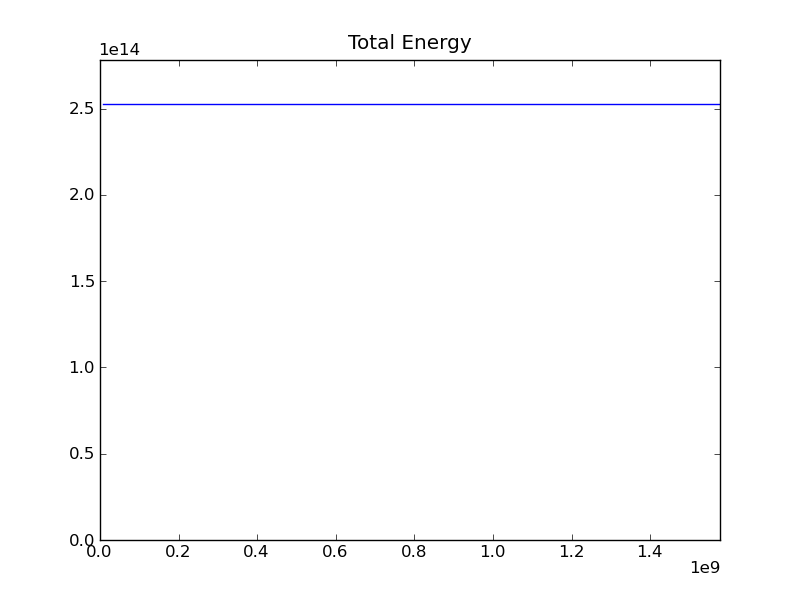
\includegraphics[width=4in]{figures/ttblockspyplot150}
\caption{Total Energy in the Blocks over Time (in seconds).}
\label{fig:onedheatout1} 
\end{center}
\end{figure}

\subsection{Plotting the Total Energy} 
\sslist{onedheatdiff001.py}

\esc does not include its own plotting capabilities. However, it is possible to use a variety of free \pyt packages for visualisation.
Two types will be demonstrated in this cookbook; \mpl\footnote{\url{http://matplotlib.sourceforge.net/}} and \verb VTK \footnote{\url{http://www.vtk.org/}} visualisation. 
The \mpl package is a component of SciPy\footnote{\url{http://www.scipy.org}} and is good for basic graphs and plots. 
For more complex visualisation tasks in particular when it comes to  two and three dimensional problems it is recommended to us more advanced tools for instance  \mayavi \footnote{\url{http://code.enthought.com/projects/mayavi/}}
which bases on the \verb|VTK| toolkit. We will discuss the usage of \verb|VTK| based 
visualization in Chapter~\ref{Sec:2DHD} where will discuss a two dimensional PDE. 

For our simple problem we have two plotting tasks: Firstly we are interested in showing the
behaviour of the total energy over time and secondly in how the temperature distribution within the block is 
developing over time. Lets start with the first task.

The trick is to create a record of the time marks and the corresponding total energies observed.
\pyt provides the concept of lists for this. Before 
the time loop is opened we create empty lists for the time marks \verb|t_list| and the total energies \verb|E_list|. 
After the new temperature as been calculated by solving the PDE we append the new time marker and total energy
to the corresponding list using the \verb|append| method. With these modifications the script looks as follows:
\begin{python}
t_list=[]
E_list=[]
# ... start iteration:
while t<tend:
      t+=h
      mypde.setValue(Y=qH+rhocp/h*T) # set variable PDE coefficients
      T=mypde.getSolution() #get the PDE solution
      totE=integrate(rhocp*T) 
      t_list.append(t)   # add current time mark to record
      E_list.append(totE) # add current total energy to record
\end{python}
To plot $t$ over $totE$ we use the \mpl a module contained within \pylab which needs to be loaded before used;
\begin{python}
import pylab as pl # plotting package.
\end{python}
Here we are not using the \verb|from pylab import *| in order to avoid name clashes for function names 
within \esc. 

The following statements are added to the script after the time loop has been completed;
\begin{python}
pl.plot(t_list,E_list)
pl.title("Total Energy")
pl.axis([0,max(t_list),0,max(E_list)*1.1])
pl.savefig("totE.png")
\end{python}
The first statement hands over the time marks and corresponding total energies to the plotter. 
The second statment is setting the title for the plot. The third statement
sets the axis ranges. In most cases these are set appropriately by the plotter.  
The last statement renders the plot and writes the 
result into the file \verb|totE.png| which can be displayed by (almost) any image viewer. 
As expected the total energy is constant over time, see \reffig{fig:onedheatout1}.

\subsection{Plotting the Temperature Distribution}
\sslist{onedheatdiff001b.py}
For plotting the spatial distribution of the temperature we need to modify the strategy we have used
for the total energy. Instead of producing a final plot at the end we will generate a 
picture at each time step which can be browsed as slide show or composed to a movie.
The first problem we encounter is that if we produce an image in each time step we need
to make sure that the images previously generated are not overwritten.

To develop an incrementing file name we can use the following convention. It is convenient to
put all image file showing the same variable - in our case the temperature distribution -
into a separate directory. As part of the \verb|os| module\footnote{The \texttt{os} module provides 
a powerful interface to interact with the operating system, see \url{http://docs.python.org/library/os.html}.} \pyt 
provides the  \verb|os.path.join| command to build file and
directory names in a platform independent way. Assuming that 
\verb|save_path| is name of directory we want to put the results the command is; 
\begin{python}
import os
os.path.join(save_path, "tempT%03d.png"%i )
\end{python}
where \verb|i| is the time step counter.
There are two arguments to the \verb join  command. The \verb save_path  variable is a predefined string pointing to the directory we want to save our data in, for example a single sub-folder called \verb data  would be defined by;
\begin{verbatim}
save_path = "data"
\end{verbatim}
while a sub-folder of \verb data  called \verb onedheatdiff001  would be defined by;
\begin{verbatim}
save_path = os.path.join("data","onedheatdiff001")
\end{verbatim}
The second argument of \verb join \xspace contains a string which is the file name or subdirectory name. We can use the operator \verb|%| to increment our file names with the value \verb|i| denoting a incrementing counter. The sub-string \verb %03d  does this by defining the following parameters; 
\begin{itemize}
 \item \verb 0  becomes the padding number;
 \item \verb 3  tells us the amount of padding numbers that are required; and
 \item \verb d  indicates the end of the \verb %  operator.
\end{itemize}
To increment the file name a \verb %i  is required directly after the operation the string is involved in. When correctly implemented the output files from this command would be place in the directory defined by \verb save_path  as;
\begin{verbatim}
blockspyplot.png
blockspyplot.png
blockspyplot.png
...
\end{verbatim}
and so on.

A sub-folder check/constructor is available in \esc. The command;
\begin{verbatim}
mkDir(save_path)
\end{verbatim}
will check for the existence of \verb save_path  and if missing, make the required directories.

We start by modifying our solution script from before.
Prior to the \verb|while| loop we will need to extract our finite solution points to a data object that is compatible with \mpl. First we create the node coordinates of the sample points used to represent
the temperature as a \pyt list of tuples or a \numpy array as requested by the plotting function. 
We need to convert thearray \verb|x| previously set as \verb|Solution(blocks).getX()| into a \pyt list 
and then to a \numpy array. The $x\hackscore{0}$ component is then extracted via an array slice to the variable \verb|plx|; 
\begin{python}
import numpy as np # array package.
#convert solution points for plotting
plx = x.toListOfTuples() 
plx = np.array(plx) # convert to tuple to numpy array
plx = plx[:,0] # extract x locations
\end{python}

\begin{figure}
\begin{center}
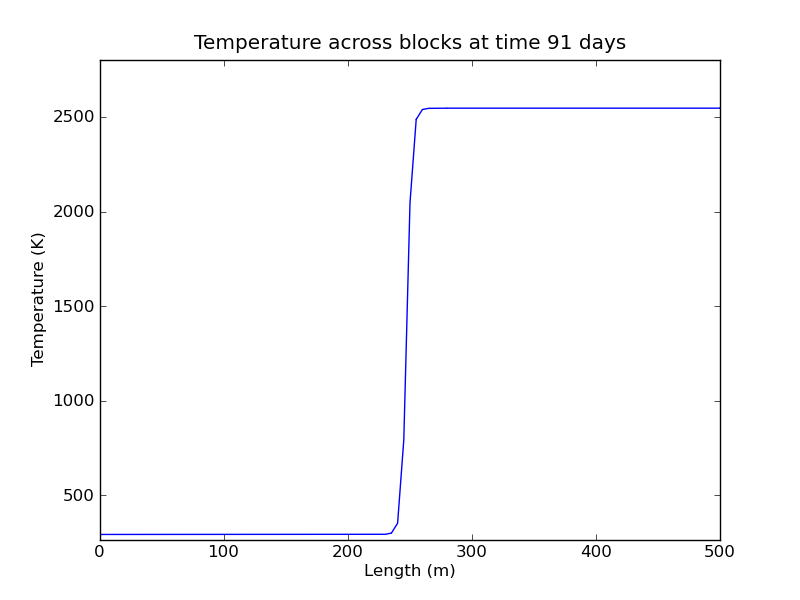
\includegraphics[width=4in]{figures/blockspyplot001}
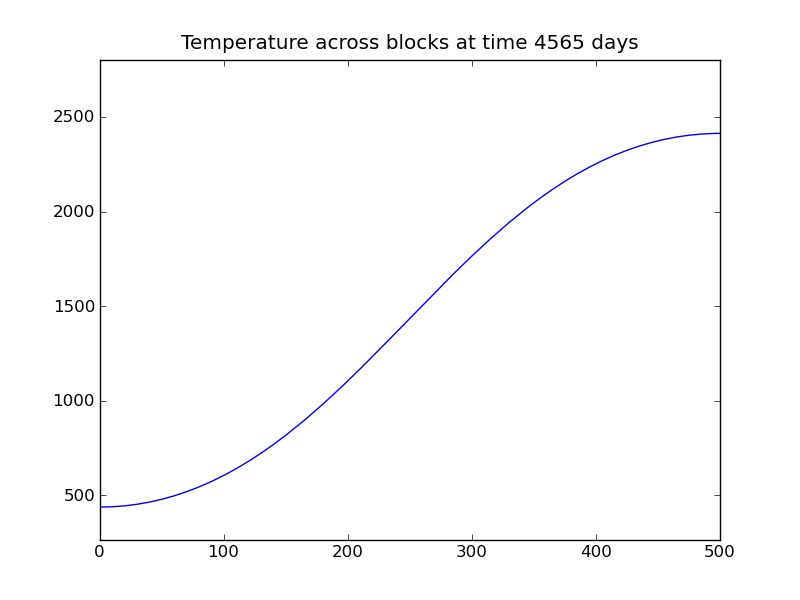
\includegraphics[width=4in]{figures/blockspyplot050}
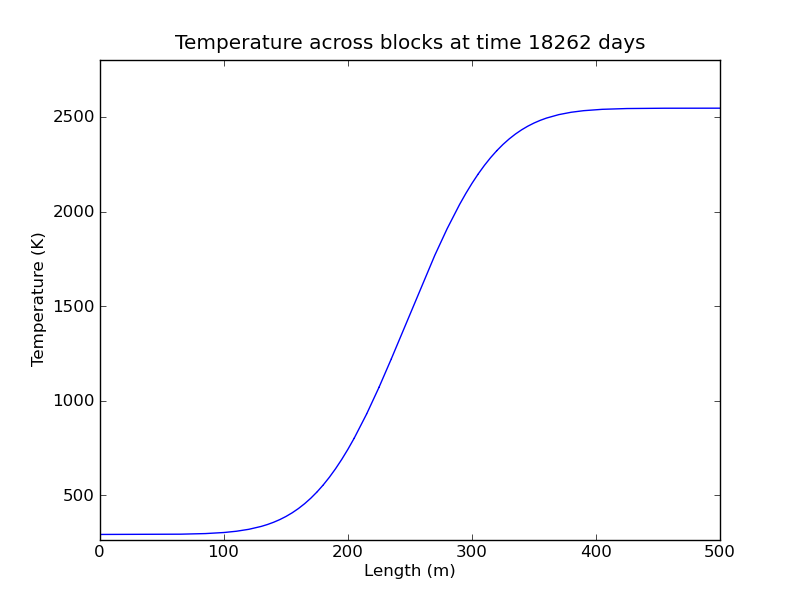
\includegraphics[width=4in]{figures/blockspyplot200}
\caption{Temperature ($T$) distribution in the blocks at time steps $1$, $50$ and $200$.}
\label{fig:onedheatout} 
\end{center}
\end{figure}

For each time step we will generate a plot of the temperature distribution and save each to a file. We use the same
techniques provided by \mpl as we have used to plot the total energy over time.
The following is appended to the end of the \verb while  loop and creates one figure of the temperature distribution. We start by converting the solution to a tuple and then plotting this against our \textit{x coordinates} \verb plx  we have generated before. We add a title to the diagram before it is rendered into a file. 
Finally, the figure is saved to a \verb|*.png| file and cleared for the following iteration.
\begin{python}
# ... start iteration:
while t<tend:
        ....
	T=mypde.getSolution() #get the PDE solution
        tempT = T.toListOfTuples() # convert to a tuple
        pl.plot(plx,tempT) # plot solution
	# set scale (Temperature should be between Tref and T0)
        pl.axis([0,mx,Tref*.9,T0*1.1])
        # add title
	pl.title("Temperature across the blocks at time %e minutes"%(t/day))
	#save figure to file
	pl.savefig(os.path.join(save_path,"tempT","blockspyplot%03d.png") %i)
\end{python}
Some results are shown in \reffig{fig:onedheatout}. 

\subsection{Make a video} 
Our saved plots from the previous section can be cast into a video using the following command appended to the end of the script. \verb mencoder  is Linux only however, and other platform users will need to use an alternative video encoder.
\begin{python}
# compile the *.png files to create a *.avi videos that show T change
# with time. This operation uses Linux mencoder. For other operating 
# systems it is possible to use your favourite video compiler to
# convert image files to videos.

os.system("mencoder mf://"+save_path+"/tempT"+"/*.png -mf type=png:\
           w=800:h=600:fps=25 -ovc lavc -lavcopts vcodec=mpeg4 -oac copy -o \
           onedheatdiff001tempT.avi")
\end{python}
 
